\documentclass{article}
\usepackage[utf8]{inputenc}
\usepackage{amsmath}
\usepackage{graphicx}
\usepackage{float}

\graphicspath {}


\title{Networks and Random Processes Assignment 1}
\author{Charlie Pilgrim - 1864704}
\date{October 2018}

\begin{document}

\maketitle


\section{Question 1}

This section considers a Simple Random Walk on ${1,...,L}$ with probabilities $p \in [0,1]$ and $q = 1-p$ to jump right and left respectively. 

Different boundary conditions are considered.

\subsection{Part A}

\subsubsection{Case 1 - Periodic}

Periodic boundary conditions, $p(0,L) = q$ and $p(L,0) = p$

The transition matrix is:

\bigskip

$P = \begin{bmatrix}
    0 & p & 0 & \dots  & 0 & q \\
    q & 0 & p & \dots  & 0 & 0\\
    0 & q & 0 & \dots  & 0 & 0\\
    \vdots & \vdots & \vdots & \ddots & \vdots \\
    0 & 0 & 0 & \dots & 0 & p \\
    p & 0 & 0 & \dots & q & 0
\end{bmatrix}$

\bigskip

The process is irreducible i.e. every state can, eventually, reach every other state. And there is a finite state space so there is 1 unique stationary distribution.

The process can "loop" around from state L to 1 and vice versa. The state path can be visualised as a circlular loop. Considering the symmetry, the stationary distribution must be uniform. 

$\pi = (1/L, 1/L,..., 1/L) \text{ for all } p \in (0,1)$ 

The stationary distribution is reversible only for the case $p=q=\frac{1}{2}$.


\subsubsection{Case 2 - Closed}

Transition matrix:

\bigskip

$P = \begin{bmatrix}
    q & p & 0 & \dots  & 0 & 0 \\
    q & 0 & p & \dots  & 0 & 0\\
    0 & q & 0 & \dots  & 0 & 0\\
    \vdots & \vdots & \vdots & \ddots & \vdots \\
    0 & 0 & 0 & \dots & 0 & p \\
    0 & 0 & 0 & \dots & q & p
\end{bmatrix}$

\bigskip

If $p = 1$ there is an absorbing state at L and the stationary distribution is $\pi = (0,0,...,0,1)$. This stationary distribution is reversible because all terms in the detailed balance equations are zero. This is not irreducible because the walk can only move from $s_x$ to $s_{x+1}$, and not in the opposite direction. 

\bigskip

If $q = 1$ there is an absorbing state at 1 and the stationary dsitribution is $\pi = (1,0,...,0,0)$. This stationary distribution is reversible because all terms in the detailed balance equations are zero. This is not irreducible, as the walk can only move from $s_x$ to $s_{x-1}$ and not in the opposite direction. 

\bigskip

If $p = q =\frac{1}{2}$ the process is irreducible because every state can, eventually, be reached from every other state. There is also a finite state space and so there is only 1 stationary distribution. All of the columns in the transition matrix sum to 1 and so there is a constant left eigenvector. Therefore the the unique stationary distribution is uniform and given by $\pi = (1/L, 1/L,..., 1/L)$. This stationary distribution is reversible.

\bigskip

If $p,q \neq [0,1/2,1]$ then the process is irreducible and it has a finite state space. So the process is ergodic and there is only 1 stationary distribution. Looking at the detailed balance equations, we can find a recurrence relation of the form:

$\pi_{x-1} p = \pi_x q \text{ over } x = \{2,3,..., L\}$


$ \pi_x = \pi_{x-1} \frac{p}{q} $

By induction, the solution is

$\pi_x = \pi_1 (\frac{p}{q})^{x-1}$

This is a reversible distribution, and so must also be stationary. As the process is ergodic, this is the unique stationary distrubution.

We can check this distribution is stationary for a closed simple random walk with 4 states

\bigskip

 $\begin{bmatrix}
    \pi_1 \\
    \pi_1\frac{p}{q} \\
    \pi_1(\frac{p}{q})^2 \\
    \pi_1(\frac{p}{q})^3 
\end{bmatrix}
\begin{bmatrix}
    q & p & 0 & 0 \\
    q & 0 & p & 0\\
    0 & q & 0 & p\\
    0 & 0 & q & p
\end{bmatrix} = 
\begin{bmatrix}
    \pi_1 \\
    \pi_1\frac{p}{q} \\
    \pi_1(\frac{p}{q})^2 \\
    \pi_1(\frac{p}{q})^3 
\end{bmatrix}$

\bigskip

The normalised stationary distribution is

$\pi_x = \dfrac{\pi_1(\frac{p}{q})^{x-1}}{\sum_i^L{\pi_i}}$

\subsection{Part B - Absorbing}

The transition matrix for a simple random walk with absorbing boundary conditions is

\bigskip

$P = \begin{bmatrix}
    1 & 0 & 0 & \dots  & 0 & 0 \\
    q & 0 & p & \dots  & 0 & 0\\
    0 & q & 0 & \dots  & 0 & 0\\
    \vdots & \vdots & \vdots & \ddots & \vdots \\
    0 & 0 & 0 & \dots & 0 & p \\
    0 & 0 & 0 & \dots & 0 & 1
\end{bmatrix}$

\bigskip

The process is not irreducible, as no other states can be reached from state 1 or state L. 

The two stationary distributions suggested by the absorbing states are

$\pi_1 = [1,0,0,...,0]$

$\pi_2 = [0,0,0,...,1]$

These can be combined linearly to give stationary distributions of the form

$\pi_0 = [a,0,0,..,0,1-a] \text{ where } a \in [0,1]$

These distributions are reversible. Looking at the detailed balance conditions:

$\pi(x)p(x,y) = \pi(y)p(y,x)$ 

All terms for all equations are zero and therefore it is reversible.

\bigskip




The absorption probability in site L is 

$h_k^L = P(X_n = L \text{ for some } n \geq 0|X_0 = k)$

or

$h_k^L = P(X_n = L | X_0 = k)$

Considering k+1, k-1, and by law of total probability:

$h_{k}^L = P(X_n = L | X_1 = k+1, X_0 = k) * p + P(X_n = L | X_1 = k-1, X_0 = k) * q $

Using the Markov property:

$h_{k}^L = P(X_n = L | X_1 = k+1) \times p + P(X_n = L | X_1 = k-1) \times q $

or

$h_{k}^L = h_{k+1}^L \times p + h_{k-1}^L \times q $

The boundary conditions are:

$h_{1}^L = 0 \text{ and } h_{L}^L = 1$

\bigskip

If $p=q$ then this recursion relation becomes 

$h_{k}^L = \dfrac{h_{k+1}^L + h_{k-1}^L}{2} $

This is linear interpolation between the two surrounding states and therefore the absorption probability is linear in k. Consdiering the boundary conditions the solution is:

$h_{k}^L = \frac{k-1}{L-1}$

\bigskip

If $p\neq q$, consider the ansatz:


$h_{k}^L = \lambda^k $

Using this ansatz the recursion relation becomes

$\lambda = p \lambda^2 + q$

This has roots:

$\lambda_1 = 1 \text{ and } \lambda_2 = q/p$



The general solution is of the form:

$h_k^L = a\lambda_1 + b\lambda_2$ 

$h_k^L = a + b(\frac{q}{p})^k$ 


Looking at the boundary conditions:

$h_1^L = 0 = a + b(\frac{q}{p})$

$h_L^L = 1 = a + b(\frac{q}{p})^L$

Subtracting the first equation from the second equation, and solving for b:

$b = \dfrac{1}{(\frac{q}{p})^{L}-\frac{q}{p}})$

$a = \dfrac{-1}{(\frac{q}{p})^{L-1}-1}$


\subsection{Part C - simulations}

A simple random walk with L=10 and closed boundary conditions was simulated 500 times, with $p=0.6$ and starting at x=1 at t=0.

\begin{figure}[H]
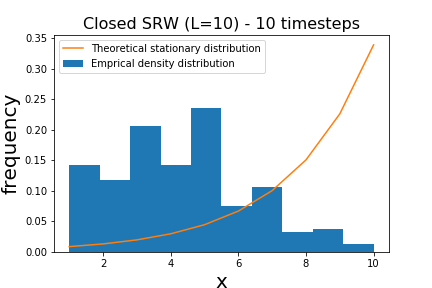
\includegraphics[scale=0.8]{10_steps_a.png} 
\small{Figure 1. The frequency distribution over 500 different realisations after 10 timesteps.}
\end{figure}

Ergodic processes tend towards the stationary distribution after a large number of time steps. After 10 time steps (Figure 1), the emprical distribution is still heavily influenced by the starting condition of x(0) = 1. 

\begin{figure}[H]
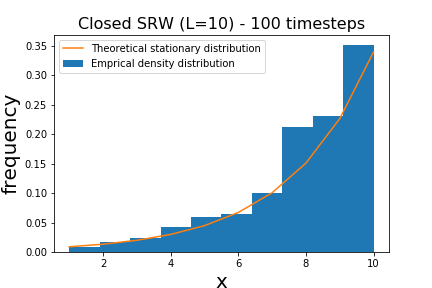
\includegraphics[scale=0.8]{100_steps_a.png} 
\small{Figure 2. The frequency distribution over 500 different realisations after 100 timesteps.}
\end{figure}

After 100 time steps (Figure 2), enough time has passed so that the empirical distribution is similar to the theoretical stationary distribution.


\begin{figure}[H]
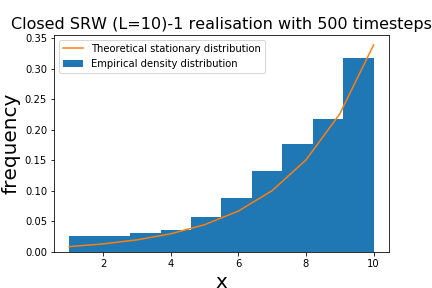
\includegraphics[scale=0.8]{500_steps_a.png} 
\small{Figure 3. The frequency distribution of states over 500 timesteps of 1 single realisations. }
\end{figure}

\begin{figure}[H]
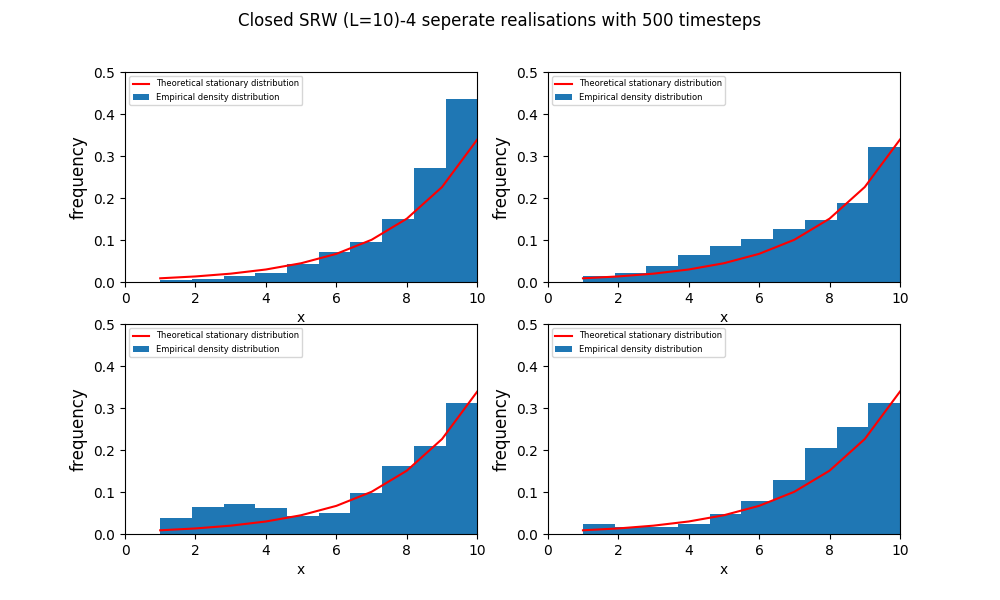
\includegraphics[scale=0.5]{500_steps_b.png} 
\small{Figure 4. The frequency distribution of states over 500 timesteps of 4 seperate single realisations. }
\end{figure}

After 500 time steps of 1 realisation (Figure 3), the empirical distribution is similar to the theoretical stationary distribution. Over just 1 realisation there is a lot of stochasticity in the specific distribution generated. To give a representative sample 4 further seperate realisations are shown in Figure 4.


\section{Question 2}

$X_1, X_2, ... $ is a sequence of independent, identically distributed random variables (iirdvs) with 

$X_i \sim N(\mu, \sigma^2)$ 

$\mu \in {R}$ and $\sigma^2 > 0$

Discrete time random walk on state space ${R}$

$(Y_n : n \geq 0)$ with $Y_{n+1} = Y_n + X_{n+1}$ and $Y_0 = 0$


\subsection{Part A}

The weak law of large numbers for $Y_n$:

$\frac{1}{n}Y_n = \frac{1}{n}\sum\limits_{k=1}^n X_k -> \mu \text{ as } n -> \infty$

The value of $\frac{Y_n}{n}$ will converge to $\mu$ with large n.

\bigskip
The central limit theorem for $Y_n$:

$\dfrac{Y_n - n\mu}{\sigma n^\frac{1}{2}} = \dfrac{1}{\sigma n^\frac{1}{2}}\sum\limits_{k=1}^n (X_k - \mu) -> \xi \text{ as } n -> \infty$

where $\xi \sim N(0,1)$

\subsection{Part B - distribution of $Y_n$}

$Y_n \sim N(n\mu, n\sigma^2) \text { for } n \geq 0$

$Y_n$ is normally distributed with mean equal to $n\mu$, where $\mu$ is the mean of the random variable $X$, and with variance $n\sigma^2$, where $\sigma^2$ is the variance of the random variable $X$. 

\subsection{Part C}

$Z_n$ has a recurive relationship given by

$Z_{n+1} = exp(Y_n + X_{n+1})$

$Z_{n+1} = Z_n exp(X_{n+1})$

\subsubsection{Derivation of pdf}

$Y$ is distributed normally, and

$Y = ln(Z)$

\bigskip

Consider the cumulative distribution function:


$F_z(z) = P(Z \leq z) = P(Y \leq ln(z)) = F_y(ln(z)) = \Phi(\dfrac{ln(z) - n\mu}{\sigma \sqrt{n}})$

$f_z(z) = \frac{d}{dz}F_z(z)$

by the chain rule, this gives

$f_z(z) = \dfrac{1}{z} \dfrac{1}{\sigma_y \sqrt{2\pi}}exp(\dfrac{-(ln(z)-\mu_y)^2}{2\sigma_y^2})$

Or, in terms of the standard deviation and mean of x

$f_z(z) = \dfrac{1}{z\sigma_x \sqrt{2n\pi}}exp(\dfrac{-(ln(z)-n\mu_x)^2}{2n\sigma_x^2})$

$Z_0$ is fixed by the initial conditions as $Z_0=1$. So the log-normal distribution given above applies for $n \geq 1$.

\bigskip

From wikipedia: 

$E(Z_n) = exp(n\mu + \frac{n\sigma^2}{2})$

$Var(Z_n) = exp(2n \mu + n\sigma^2)(exp(n\sigma^2)-1)$

$Med(Z_n) = exp(n\mu)$

Where $\mu$ and $\sigma^2$ are the mean and variance of X.

\subsection{Part D}
$Z_n$ was simulated 500 times over 100 timesteps with $\mu_x=0$ and $\sigma_x=0.2$.

\subsubsection{Empirical Average}

\begin{figure}[H]
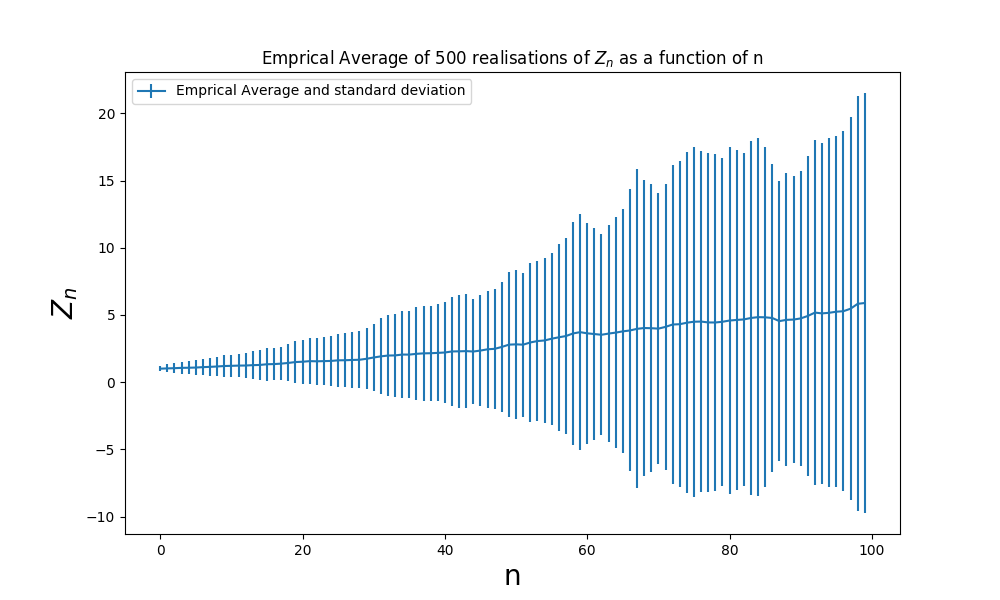
\includegraphics[scale=0.5]{empirical_average_1.png} 
\small{Figure 5. The emprical average of 500 simulations of $Z_n$ as a funciton of n over 100 timesteps. }
\end{figure}


Figure shows the empirical average of $Z_n$ as a function of time, $n$. The error bars show the emprical standard deviation at each point. 

\subsubsection{Boxplots}

\begin{figure}[H]
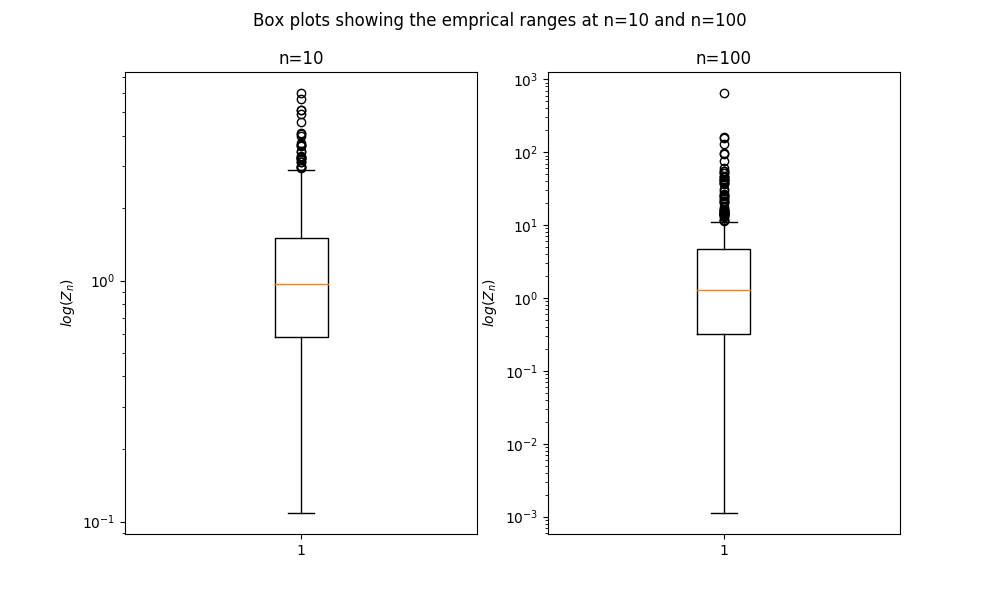
\includegraphics[scale=0.5]{box_plots_a.png} 
\small{Figure 6. The empirical ranges of $Z_n$ over 500 realisations at n=10 and n=100. The whiskers are set at $1.5 \times IQR$ where IQR is the interquartile range.}
\end{figure}

Figure 6 shows the ranges of empirical data at 10 and 100 timesteps. The distribution at 100 timesteps has a much larger range than at 10 timesteps.

\subsubsection{Emprical PDF and theoretical PDF}

\begin{figure}[H]
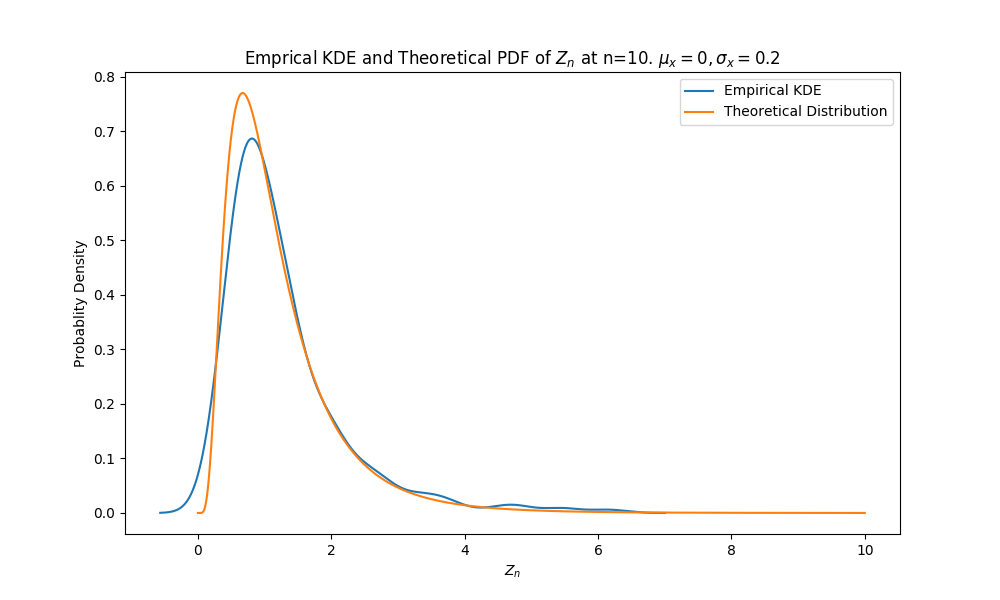
\includegraphics[scale=0.5]{empirical_pdf_kde_10_a.png} 
\small{Figure 7. Empirical kernel density estimation and theoretical probability density fucntion for $Z_n$ with $\mu_x=0$ and $\sigma=0.2$ at $n=10$ timesteps over 500 realisations.}
\end{figure}

Figure 7 shows a reasonably close fit between the empirical kernel density estimate and the theoretical probability density function for $Z_n$ at $n=10$ timesteps for 500 realisations. The closeness of the fit improves with more realisations.

TO DO - ADD IN FIG 8 FROM UNI LAPTOP


\subsubsection{Ergodic Average}

\begin{figure}[H]
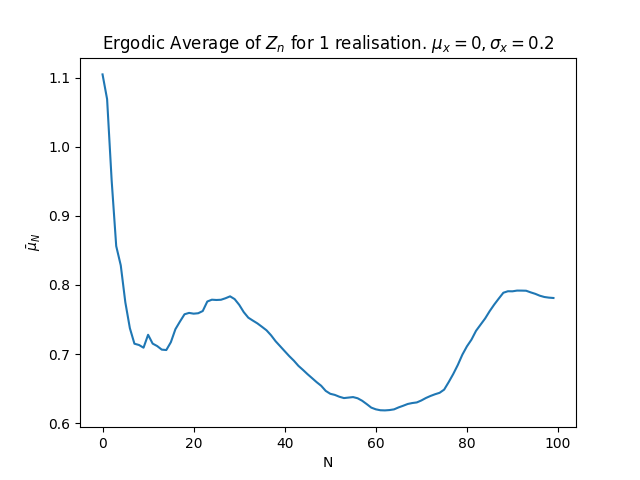
\includegraphics[scale=0.8]{ergodic_average_a.png} 
\small{Figure 9. Ergodic average of $Z_n$ for a single realisation as a function of total timesteps, N. $\mu_x=0$ and $\sigma_x=0.2$.}
\end{figure}

Figure shows the ergodic average for a single realisation plotted over 100 timsteps. 

\subsection{Part E - Empirical Tail}

$E(Z_n) = 1 \text{ for all } n\geq0$

$E(Z_n) = exp(n\mu + \frac{n\sigma^2}{2}) = 1$

$\mu + \frac{\sigma^2}{2} = 0$

$\mu = - \frac{\sigma^2}{2}$

$\mu = -\frac{1}{50}$

A value of $\mu_x$ of -0.02 will give $E(Z_n)=1$ for all $n \geq 0$.

\begin{figure}[H]
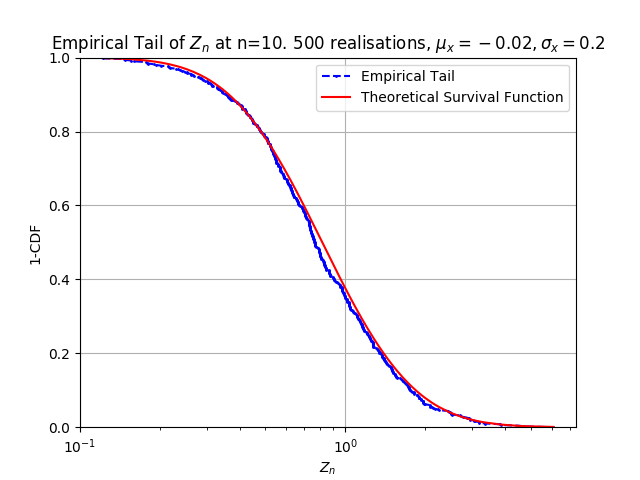
\includegraphics[scale=0.8]{empirical_tail_10_a.png} 
\small{Figure 10. Empirical tail of $Z_n$ compared to the theoretical prediction of the survival function, 1-Cumulative Density Function. At timestep 10. 500 realisations, $\mu_x=-0.02$, $\sigma_x=0.02$.}
\end{figure}


\begin{figure}[H]
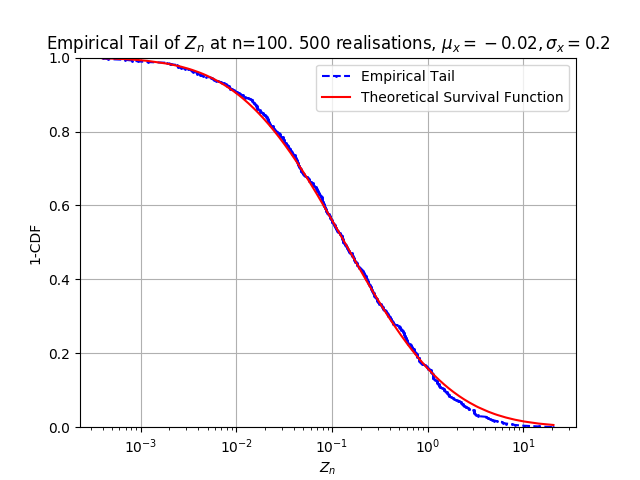
\includegraphics[scale=0.8]{empirical_tail_100_a.png} 
\small{Figure 11. Empirical tail of $Z_n$ compared to the theoretical prediction of the survival function, 1-Cumulative Density Function. At timestep 100. 500 realisations, $\mu_x=-0.02$, $\sigma_x=0.02$.}
\end{figure}

Figures 10 and 11 show the empirical tail of $Z_n$ at timesteps $n=10$ and $n=100$ respectively, with a close fit to the theoretical prediction. 




Figure shows the emprical tail of the data compared to the theoretical survival function, defined as 1 minus the cumulative distribution function.


\subsection{Part f}

As $n-> \infty$, the $E(Z_n)$ remains at 1 but the variance continues to grow, so $Z_n$ can be found anywhere. The distribution of $Z_n$ is flattened out as n grows, and so there is not a unique stationary distribution and the process is not ergodic. 

By the law of large numbers, the emprical average

$\hat{\mu}^M = \frac{1}{M} \sum_{i=1}^{M}Z_n^i -> E(Z_n) \text{ as } M -> \infty$

$E(Z_n) = 1$

Therefore, as $M -> \infty$, the empricial average should converge to 1 for fixed n.

At very large n, the expected value of $Z_n$ is still 1, so for fixed finite M  

$\hat{\mu}_n^M -> \frac{1}{M} \text{ as } n -> \infty$

\bigskip

The limits do not commute

$\lim\limits_{n\to\infty} \lim\limits_{M\to\infty} \hat{\mu}_n^M \neq \lim\limits_{M\to\infty} \lim\limits_{m\to\infty} \hat{\mu}_n^M$

$\lim\limits_{n\to\infty} 1 \neq \lim\limits_{M\to\infty} \frac{1}{M}$

$1 \neq 0$
 
\bigskip

The limit of $\bar{\mu}_N$ as $N\to\infty$ is equivalent to the right hand side of the previous limit equation, so is converges to 0. Thie does not contradict the ergdoic theorem, which would suggest it converges to 1, because there is not a unique stationary distribution and so the Ergdoic theorem does not apply. 
 




\section{Question 3}

\subsection{Part a}

Each individual can have the starting type of any other individual. Let $T$ equal the set of all unique starting states, so 

$T = \{X_0(1), X_0(2), . . . , X_0(L)\}$

Each individual can have a type of any element in that set. This gives a total state space of size $L^2$. In mathematical notation:

$X(i) \in T \quad \forall \, i \in \{1,2,...,L\}$ 


$X(i) \in \{X_0(1), X_0(2), . . . , X_0(L)\} \quad \forall \, i \in \{1,2,...,L\}$ 

$X(i) \in X_0(j) \text{ where } \ j \in \{1,2,...,L\} \quad \forall \, i \in\{1,2,...,L\}$ 


The process is not irreducible, as once a type goes extinct it stays extinct, and so not every state can be reached from every other state.

The stationary distributions are where all individuals are of one type i.e. all $X(i)$ are equal to the same one of the initial types $X_0(j)$. In mathematical notation:

$ X(i) = X_0(j) \text{ where } j \in \{1,2,..,L\}$

\subsection{Part b}

\subsubsection{State space}

The future state of the process depends only on the current state at each time step, so yes it is Markov. 

The state space is 

$N \in \{0,1,...,L\} $ 

For each type, there can be an integer number of individuals of that type between 0 and L. 

\subsubsection{Transition Probabilities}

Let $N_t(j)$ be the number of individuals of a particular species, $j$ in a generation, and L individuals in total. For indiviudal of the next generation, the probability of being of this particular species is equal to the proportion of individuals of that type in the parent generation. 

$p(X_{t+1}(i) = j) = N_t(j)/L$

So the transition probabilites for $N_t+1$ are given by a binomial distribution:

$p(N_{t+1}(j) = k) = {L \choose k}(\frac{N_t(j)}{L})^k(1-\frac{N_t(j)}{L})^{L-k} \text{ , } \quad k=0,1,...,L$

The process is not irreducible, if the number of indiviudals of the given species reaches zero, then it is extinct and can never grow again above zero. If the number of individuals reaches L, then this species is the only species left and will always remain so. 

\subsubsection{Stationary Distributions}

If we define a distribution vector as

$\pi = [N_t(0), N_t(1),...,N_t(L)]$

Then there are stationary distributions on the absorbing states

$\pi_1 = [1, 0,...,0,0]$

$\pi_2 = [0, 0,...,0,1]$

and any normalised linear combination of these states, so

$\pi_0 = [a, 0,...,0,1-a] \text{ where } a \in [0,1]$ 

With the initial condition $N_0 = 1$, there is one individual of this type in the population. By symmetry, the probability of this species taking over has to be equal to $1/L$. So the limiting distribution as $t -> \infty$ is

$\pi_{\infty} = [1-\frac{1}{L},0,...,0,\frac{1}{L}]$



The process is not irreducible, as once a state has $N_i = 0$ for any i, i.e. a type goes extinct, the state space where $N_i >0$ is no longer accessible.


\subsection{Part C - Simulations}

\begin{figure}[H]
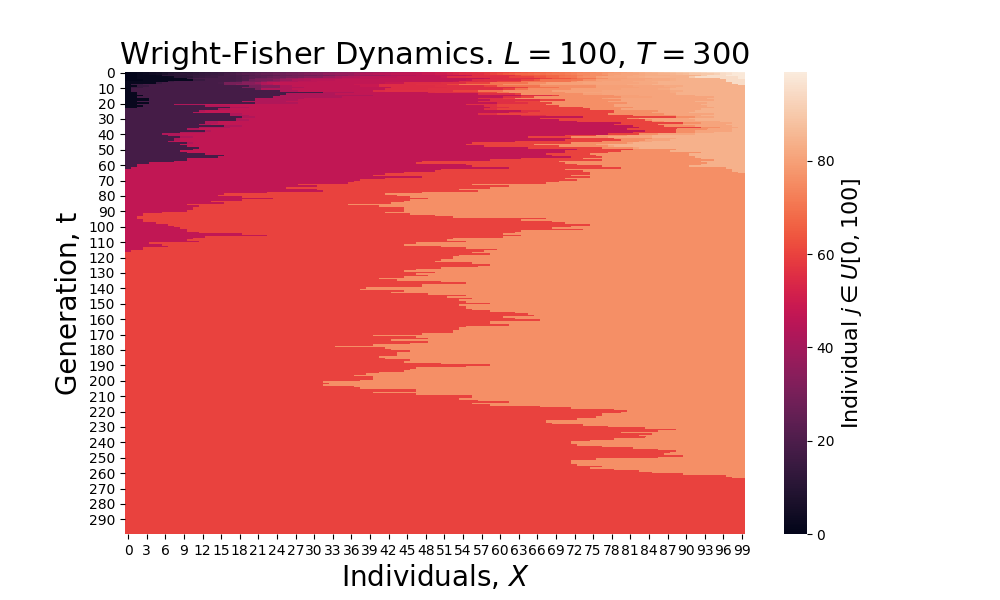
\includegraphics[scale=0.6]{Wright-Fisher_a.png} 
\small{Figure 12. Dynamics of Wright-Fisher model of population dynamics with $L=100$ individuals of unique type at generation $t=0$.}
\end{figure}


In this simulation there is only one type left after about 260 generations. In the earlier generations, the number of types is quickly reduced as types go extinct. In this simulation there are only 3 types left after about 70 generations. 

The probability of any particular type going extinct in the next generation is

$p(N_{t+1}(j) = 0) = (1-\frac{N_t(j)}{L})^{L}$


If there is only one individual left, as in generation 0, then this is approximately 0.37. In later generations, there are often many individuals of a surviving type, and so the chance of that type going extinct is lower, but non-zero.

While there is more than one type, there is always a probability that one or more of the types will go extinct in the following generation. So over time the number of unique generations reduces. Given enough time, the number of types will always go to 1. 


\begin{figure}[H]
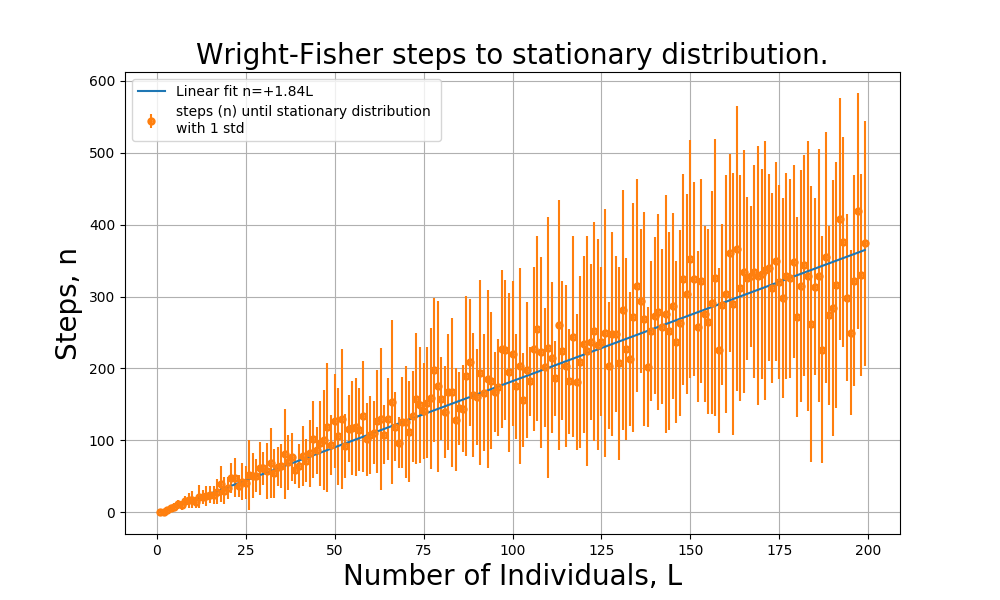
\includegraphics[scale=0.5]{Wright_Fisher_absorption_a.png} 
\small{Figure 13. Average time to absorption for Wright-Fisher model as a function of number of individuals. Each L was simulated 20 times, with the empirical average and 1 standard deviation shown.}
\end{figure}

Figure shows an empirical simulation of the time to absorption, $n_{abs}$ as a function of the number of individuals. There appears to be a linear relationship, approximately of the form:

$n_{abs} = 1.84L $

This is an approximate relationship and further work should be done to determine the confidence interval.

\end{document}





